% Options for packages loaded elsewhere
\PassOptionsToPackage{unicode}{hyperref}
\PassOptionsToPackage{hyphens}{url}
%
\documentclass[
]{book}
\usepackage{amsmath,amssymb}
\usepackage{lmodern}
\usepackage{iftex}
\ifPDFTeX
  \usepackage[T1]{fontenc}
  \usepackage[utf8]{inputenc}
  \usepackage{textcomp} % provide euro and other symbols
\else % if luatex or xetex
  \usepackage{unicode-math}
  \defaultfontfeatures{Scale=MatchLowercase}
  \defaultfontfeatures[\rmfamily]{Ligatures=TeX,Scale=1}
\fi
% Use upquote if available, for straight quotes in verbatim environments
\IfFileExists{upquote.sty}{\usepackage{upquote}}{}
\IfFileExists{microtype.sty}{% use microtype if available
  \usepackage[]{microtype}
  \UseMicrotypeSet[protrusion]{basicmath} % disable protrusion for tt fonts
}{}
\makeatletter
\@ifundefined{KOMAClassName}{% if non-KOMA class
  \IfFileExists{parskip.sty}{%
    \usepackage{parskip}
  }{% else
    \setlength{\parindent}{0pt}
    \setlength{\parskip}{6pt plus 2pt minus 1pt}}
}{% if KOMA class
  \KOMAoptions{parskip=half}}
\makeatother
\usepackage{xcolor}
\usepackage{color}
\usepackage{fancyvrb}
\newcommand{\VerbBar}{|}
\newcommand{\VERB}{\Verb[commandchars=\\\{\}]}
\DefineVerbatimEnvironment{Highlighting}{Verbatim}{commandchars=\\\{\}}
% Add ',fontsize=\small' for more characters per line
\usepackage{framed}
\definecolor{shadecolor}{RGB}{248,248,248}
\newenvironment{Shaded}{\begin{snugshade}}{\end{snugshade}}
\newcommand{\AlertTok}[1]{\textcolor[rgb]{0.94,0.16,0.16}{#1}}
\newcommand{\AnnotationTok}[1]{\textcolor[rgb]{0.56,0.35,0.01}{\textbf{\textit{#1}}}}
\newcommand{\AttributeTok}[1]{\textcolor[rgb]{0.77,0.63,0.00}{#1}}
\newcommand{\BaseNTok}[1]{\textcolor[rgb]{0.00,0.00,0.81}{#1}}
\newcommand{\BuiltInTok}[1]{#1}
\newcommand{\CharTok}[1]{\textcolor[rgb]{0.31,0.60,0.02}{#1}}
\newcommand{\CommentTok}[1]{\textcolor[rgb]{0.56,0.35,0.01}{\textit{#1}}}
\newcommand{\CommentVarTok}[1]{\textcolor[rgb]{0.56,0.35,0.01}{\textbf{\textit{#1}}}}
\newcommand{\ConstantTok}[1]{\textcolor[rgb]{0.00,0.00,0.00}{#1}}
\newcommand{\ControlFlowTok}[1]{\textcolor[rgb]{0.13,0.29,0.53}{\textbf{#1}}}
\newcommand{\DataTypeTok}[1]{\textcolor[rgb]{0.13,0.29,0.53}{#1}}
\newcommand{\DecValTok}[1]{\textcolor[rgb]{0.00,0.00,0.81}{#1}}
\newcommand{\DocumentationTok}[1]{\textcolor[rgb]{0.56,0.35,0.01}{\textbf{\textit{#1}}}}
\newcommand{\ErrorTok}[1]{\textcolor[rgb]{0.64,0.00,0.00}{\textbf{#1}}}
\newcommand{\ExtensionTok}[1]{#1}
\newcommand{\FloatTok}[1]{\textcolor[rgb]{0.00,0.00,0.81}{#1}}
\newcommand{\FunctionTok}[1]{\textcolor[rgb]{0.00,0.00,0.00}{#1}}
\newcommand{\ImportTok}[1]{#1}
\newcommand{\InformationTok}[1]{\textcolor[rgb]{0.56,0.35,0.01}{\textbf{\textit{#1}}}}
\newcommand{\KeywordTok}[1]{\textcolor[rgb]{0.13,0.29,0.53}{\textbf{#1}}}
\newcommand{\NormalTok}[1]{#1}
\newcommand{\OperatorTok}[1]{\textcolor[rgb]{0.81,0.36,0.00}{\textbf{#1}}}
\newcommand{\OtherTok}[1]{\textcolor[rgb]{0.56,0.35,0.01}{#1}}
\newcommand{\PreprocessorTok}[1]{\textcolor[rgb]{0.56,0.35,0.01}{\textit{#1}}}
\newcommand{\RegionMarkerTok}[1]{#1}
\newcommand{\SpecialCharTok}[1]{\textcolor[rgb]{0.00,0.00,0.00}{#1}}
\newcommand{\SpecialStringTok}[1]{\textcolor[rgb]{0.31,0.60,0.02}{#1}}
\newcommand{\StringTok}[1]{\textcolor[rgb]{0.31,0.60,0.02}{#1}}
\newcommand{\VariableTok}[1]{\textcolor[rgb]{0.00,0.00,0.00}{#1}}
\newcommand{\VerbatimStringTok}[1]{\textcolor[rgb]{0.31,0.60,0.02}{#1}}
\newcommand{\WarningTok}[1]{\textcolor[rgb]{0.56,0.35,0.01}{\textbf{\textit{#1}}}}
\usepackage{longtable,booktabs,array}
\usepackage{calc} % for calculating minipage widths
% Correct order of tables after \paragraph or \subparagraph
\usepackage{etoolbox}
\makeatletter
\patchcmd\longtable{\par}{\if@noskipsec\mbox{}\fi\par}{}{}
\makeatother
% Allow footnotes in longtable head/foot
\IfFileExists{footnotehyper.sty}{\usepackage{footnotehyper}}{\usepackage{footnote}}
\makesavenoteenv{longtable}
\usepackage{graphicx}
\makeatletter
\def\maxwidth{\ifdim\Gin@nat@width>\linewidth\linewidth\else\Gin@nat@width\fi}
\def\maxheight{\ifdim\Gin@nat@height>\textheight\textheight\else\Gin@nat@height\fi}
\makeatother
% Scale images if necessary, so that they will not overflow the page
% margins by default, and it is still possible to overwrite the defaults
% using explicit options in \includegraphics[width, height, ...]{}
\setkeys{Gin}{width=\maxwidth,height=\maxheight,keepaspectratio}
% Set default figure placement to htbp
\makeatletter
\def\fps@figure{htbp}
\makeatother
\setlength{\emergencystretch}{3em} % prevent overfull lines
\providecommand{\tightlist}{%
  \setlength{\itemsep}{0pt}\setlength{\parskip}{0pt}}
\setcounter{secnumdepth}{5}
\usepackage{booktabs}
\usepackage[version=4]{mhchem} 
\usepackage{siunitx}
\newcommand{\conc}[1]{\left[ \ce{#1} \right]}
\usepackage{booktabs}
\usepackage{longtable}
\usepackage{array}
\usepackage{multirow}
\usepackage{wrapfig}
\usepackage{float}
\usepackage{colortbl}
\usepackage{pdflscape}
\usepackage{tabu}
\usepackage{threeparttable}
\usepackage{threeparttablex}
\usepackage[normalem]{ulem}
\usepackage{makecell}
\usepackage{xcolor}
\ifLuaTeX
  \usepackage{selnolig}  % disable illegal ligatures
\fi
\usepackage[]{natbib}
\bibliographystyle{plainnat}
\IfFileExists{bookmark.sty}{\usepackage{bookmark}}{\usepackage{hyperref}}
\IfFileExists{xurl.sty}{\usepackage{xurl}}{} % add URL line breaks if available
\urlstyle{same} % disable monospaced font for URLs
\hypersetup{
  pdftitle={Resumen de clases},
  pdfauthor={J. Clavijo \& E. Romero},
  hidelinks,
  pdfcreator={LaTeX via pandoc}}

\title{Resumen de clases}
\author{J. Clavijo \& E. Romero}
\date{2022-07-08}

\usepackage{amsthm}
\newtheorem{theorem}{Teorema}[chapter]
\newtheorem{lemma}{Lema}[chapter]
\newtheorem{corollary}{Corolario}[chapter]
\newtheorem{proposition}{Proposición}[chapter]
\newtheorem{conjecture}{Conjecture}[chapter]
\theoremstyle{definition}
\newtheorem{definition}{Definición}[chapter]
\theoremstyle{definition}
\newtheorem{example}{Ejemplo}[chapter]
\theoremstyle{definition}
\newtheorem{exercise}{Ejercicio}[chapter]
\theoremstyle{definition}
\newtheorem{hypothesis}{Hypothesis}[chapter]
\theoremstyle{remark}
\newtheorem*{remark}{Nota: }
\newtheorem*{solution}{Solución}
\begin{document}
\maketitle

{
\setcounter{tocdepth}{1}
\tableofcontents
}
\begin{Shaded}
\begin{Highlighting}[]
\FunctionTok{library}\NormalTok{(tidyverse)}
\FunctionTok{library}\NormalTok{(kableExtra)}
\end{Highlighting}
\end{Shaded}

\hypertarget{acerca}{%
\chapter*{Acerca}\label{acerca}}
\addcontentsline{toc}{chapter}{Acerca}

Este libro incluye el resumen de las clases de principios de análisis químico, al igual que la ampliación de los ejercicios trabajados en clase. sdf

\hypertarget{uso}{%
\section*{Uso}\label{uso}}
\addcontentsline{toc}{section}{Uso}

Cada capítulo contendrá los diferentes temas vistos en clase divididos de acuerdo al programa calendario.

También incoporará la solución de ejercicios con la calculadora HP 48gx y 50g, al igual que en R.

\hypertarget{alcance}{%
\section*{Alcance}\label{alcance}}
\addcontentsline{toc}{section}{Alcance}

Este no pretende reemplazar los libros recomendados para la asignatura sino que es una material de apoyo para el estudio de los estudiantes de la asignatura de principios de análisis químico.

\hypertarget{cantidades-fuxedsicas-y-cuxe1lculo-de-cantidades}{%
\chapter{Cantidades físicas y cálculo de cantidades}\label{cantidades-fuxedsicas-y-cuxe1lculo-de-cantidades}}

El valor de una cantidad física Q puede expresarse como el producto de un valor numérico \{Q\} y una unidad {[}Q{]}
\[ Q = \{Q\}\ [Q]\]
ni el nombre de la cantidad física, ni el símbolo utilizado para denotarla, implican una elección particular de la unidad \footnote{El símbolo {[}Q{]} se utilizaba antes para la dimensión de Q, pero este símbolo se utiliza y se prefiere para la unidad de Q.}.

Las cantidades físicas, los valores numéricos y las unidades pueden manipularse con las reglas ordinarias del álgebra. Así podemos escribir, por ejemplo, para la longitud de onda \(\lambda\) de una de las líneas amarillas de sodio.
\begin{equation} 
  \lambda = 5.896\times 10^{-7}\text{ m} = 589.6\text{ nm}
  \label{eq:lineasodio}
\end{equation}

donde m es el símbolo de la unidad de longitud llamada metro, nm es el símbolo del nanómetro, y las unidades metro y nanómetro están relacionadas por:
\begin{equation} 
  1\text{ nm} = 10^{-9}\text{ m}
  \label{eq:relacionnmmetro}
\end{equation}
La equivalencia de las dos expresiones para \(\lambda\) en la ecuación \eqref{eq:lineasodio} se deduce de inmediato cuando tratamos las unidades según las reglas del álgebra y reconocemos la identidad de \(1 \text{ nm}\) y \(10^{-9} \text{ m}\) en la ecuación \eqref{eq:relacionnmmetro}. La longitud de onda puede expresarse igualmente en la forma:
\begin{equation} 
  \lambda/\text{m} = 5.896\times 10^{-7}
  \label{eq:despejemetro}
\end{equation}
o
\begin{equation} 
  \lambda/\text{nm} = 589.6
  \label{eq:despejenanometro}
\end{equation}
Puede ser útil trabajar con variables que se definen dividiendo la cantidad por una unidad determinada. Por ejemplo, al tabular los valores numéricos de las magnitudes físicas o al etiquetar los ejes de los gráficos, es especialmente conveniente utilizar el cociente de una magnitud física y una unidad de forma que los valores a tabular sean valores numéricos, como en las ecuaciones \eqref{eq:despejemetro} y \eqref{eq:despejenanometro}.

\begin{table}

\caption{\label{tab:examplequantity}Recreating booktabs style table}
\centering
\begin{tabular}[t]{r|r|r|r}
\hline
\$T/\textbackslash{}text\{K\}\$ & \$10\textasciicircum{}\{3\}\textbackslash{} \textbackslash{}text\{K\}/T\$ & \$p/\textbackslash{}text\{MPa\}\$ & \$\textbackslash{}ln \textbackslash{}left(p/\textbackslash{}text\{MPa\}\textbackslash{}right)\$\\
\hline
216.55 & 4.6179 & 0.5180 & -0.6578\\
\hline
273.15 & 3.6610 & 3.4853 & 1.2486\\
\hline
304.19 & 3.2874 & 7.3815 & 1.9990\\
\hline
\end{tabular}
\end{table}

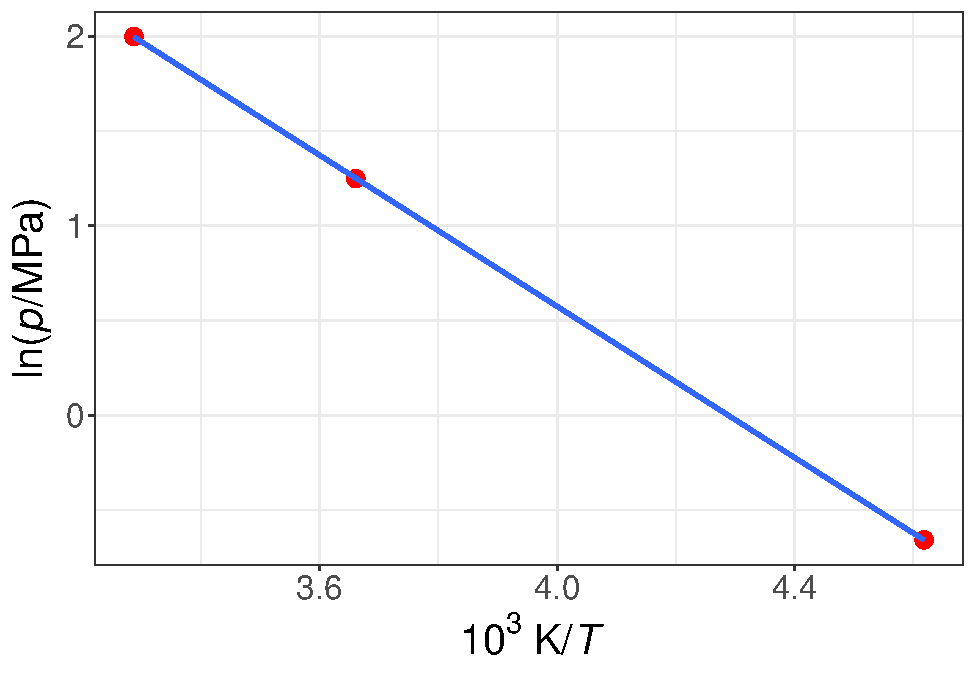
\includegraphics{PAQ_BOOK_files/figure-latex/examplequantity-1.pdf}

\hypertarget{equilibrio-uxe1cido-base}{%
\chapter{Equilibrio ácido-base}\label{equilibrio-uxe1cido-base}}

\hypertarget{soluciones-reguladoras}{%
\section{Soluciones reguladoras}\label{soluciones-reguladoras}}

\emph{Una solución amortiguadora (regulada o buffer) se opone a cambios de pH cuando se le añaden ácidos o bases, o cuando se diluye}. Una solución reguladora está compúesta por la mezcla de un ácido débil y su base conjugada ó una base débil y su ácido conjugado, en esta mezcla el ácido y su base conjugada deben estar en cantidades comparables (dentro de una proporción de 1:10 ó 10:1) para funcionar eficazmente. Esto quiere decir que para preparar una solución reguladora existen principalmente tres opciones diferentes.

\begin{example}
Se mezcla un ácido débil y una base fuerte, pero debe cumplir que \(c(\ce{HA}) > c(\ce{NaOH})\).
\end{example}

\begin{example}
Se mezcla un ácido débil y una sal del ácido débil, pero debe cumplir que \(c(\ce{HA}) \approx c(\ce{NaA})\).
\end{example}

\begin{example}
Por último la opción menos usada es mezclar la sal del ácido débil y un ácido fuerte, pero debe cumplir que \(c(\ce{NaA}) > c(\ce{HCl})\).
\end{example}

\begin{table}

\caption{\label{tab:tables-common-buffers}Algunos reguladores comunes}
\centering
\begin{tabular}[t]{l|l}
\hline
Solución reguladora & Rango aproximado de pH\\
\hline
Ácido ftálico/hidrogeno ftalato de potasio & 2.2 - 3.8\\
\hline
Ácido acético/acetato de sodio & 3.4 - 5.9\\
\hline
Hidrogeno ftalato de potasio/ftalato de potasio & 4.0 - 6.2\\
\hline
Dihidrógeno fosfato de potasio/hidrógeno fosfato de potasio & 5.8 - 8.0\\
\hline
Ácido bórico/borato de sodio & 7.8 - 10.0\\
\hline
Glicina/glicinato de sodio & 9.5 - 11.7\\
\hline
Hidrógeno fosfato de potasio/fosfato de potasio & 11.0 - 12.0\\
\hline
\end{tabular}
\end{table}

\hypertarget{capacidad-reguladora}{%
\subsection{Capacidad reguladora}\label{capacidad-reguladora}}

La capacidad de un regulador, \(\beta\), es una medida de la resistencia de la disolución a cambiar de pH, cuando se le añade un ácido o una base fuerte. La capacidad de un regulador se define como \citep{VanSlyke1922}:

\[\beta = \frac{d\ c(\text{b})}{d \text{ pH}} = - \frac{d\ c(\text{a})}{d \text{ pH}}\]

donde \(c(\text{a})\) y \(c(\text{b})\) es la cantidad de sustancia de ácido fuerte (por ejemplo, \(n(\ce{HNO3}\))) y de base fuerte (por ejemplo, \(n(\ce{NaOH})\)) por litro necesaria para producir un cambio de una unidad de pH. Cuanto mayor es el valor de \(\beta\), más resistente es el regulador a un cambio de pH.

Para un ácido débil monoprótico la capacidad reguladora será:

\[\beta = \ln\left(10\right) \left([\ce{H3O+}] +[\ce{HO-}] + c(\ce{HA})_{Total} \times \alpha_0 \times \alpha_1 \right) \]
donde \(\alpha_0\) y \(\alpha_1\) corresponden a la especie ácida y su base conjugada, respectivamente. Para un ácido poliprótico cambia la ecuación a:

\[\beta = \ln\left(10\right) \left([\ce{H3O+}] + [\ce{HO-}] + c(\ce{HA})_{Total} \times \sum_{i=0}^{n-1} \sum_{j = i+1}^n \left(j-i\right)^2 \alpha_i \times \alpha_j \right) \]

\hypertarget{cross}{%
\chapter{Cross-references}\label{cross}}

Cross-references make it easier for your readers to find and link to elements in your book.

\hypertarget{chapters-and-sub-chapters}{%
\section{Chapters and sub-chapters}\label{chapters-and-sub-chapters}}

There are two steps to cross-reference any heading:

\begin{enumerate}
\def\labelenumi{\arabic{enumi}.}
\tightlist
\item
  Label the heading: \texttt{\#\ Hello\ world\ \{\#nice-label\}}.

  \begin{itemize}
  \tightlist
  \item
    Leave the label off if you like the automated heading generated based on your heading title: for example, \texttt{\#\ Hello\ world} = \texttt{\#\ Hello\ world\ \{\#hello-world\}}.
  \item
    To label an un-numbered heading, use: \texttt{\#\ Hello\ world\ \{-\#nice-label\}} or \texttt{\{\#\ Hello\ world\ .unnumbered\}}.
  \end{itemize}
\item
  Next, reference the labeled heading anywhere in the text using \texttt{\textbackslash{}@ref(nice-label)}; for example, please see Chapter \ref{cross}.

  \begin{itemize}
  \tightlist
  \item
    If you prefer text as the link instead of a numbered reference use: \protect\hyperlink{cross}{any text you want can go here}.
  \end{itemize}
\end{enumerate}

\hypertarget{captioned-figures-and-tables}{%
\section{Captioned figures and tables}\label{captioned-figures-and-tables}}

Figures and tables \emph{with captions} can also be cross-referenced from elsewhere in your book using \texttt{\textbackslash{}@ref(fig:chunk-label)} and \texttt{\textbackslash{}@ref(tab:chunk-label)}, respectively.

See Figure \ref{fig:nice-fig}.

\begin{Shaded}
\begin{Highlighting}[]
\FunctionTok{par}\NormalTok{(}\AttributeTok{mar =} \FunctionTok{c}\NormalTok{(}\DecValTok{4}\NormalTok{, }\DecValTok{4}\NormalTok{, .}\DecValTok{1}\NormalTok{, .}\DecValTok{1}\NormalTok{))}
\FunctionTok{plot}\NormalTok{(pressure, }\AttributeTok{type =} \StringTok{\textquotesingle{}b\textquotesingle{}}\NormalTok{, }\AttributeTok{pch =} \DecValTok{19}\NormalTok{)}
\end{Highlighting}
\end{Shaded}

\begin{figure}

{\centering 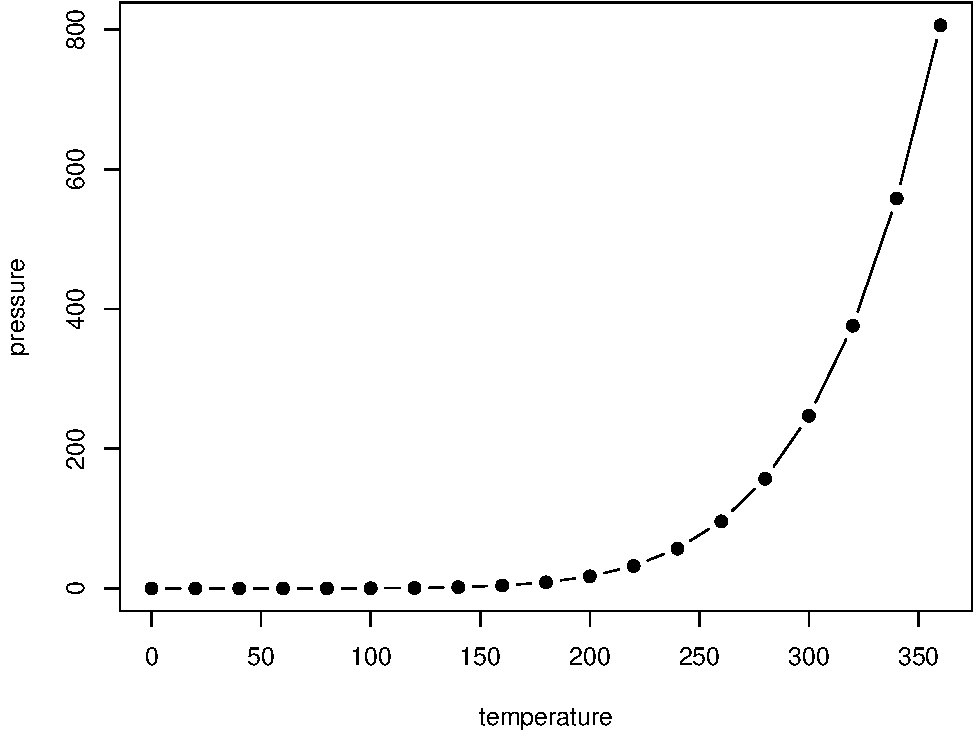
\includegraphics[width=0.8\linewidth]{PAQ_BOOK_files/figure-latex/nice-fig-1} 

}

\caption{Here is a nice figure!}\label{fig:nice-fig}
\end{figure}

Don't miss Table \ref{tab:nice-tab}.

\begin{Shaded}
\begin{Highlighting}[]
\NormalTok{knitr}\SpecialCharTok{::}\FunctionTok{kable}\NormalTok{(}
  \FunctionTok{head}\NormalTok{(pressure, }\DecValTok{10}\NormalTok{), }\AttributeTok{caption =} \StringTok{\textquotesingle{}Here is a nice table!\textquotesingle{}}\NormalTok{,}
  \AttributeTok{booktabs =} \ConstantTok{TRUE}
\NormalTok{)}
\end{Highlighting}
\end{Shaded}

\begin{table}

\caption{\label{tab:nice-tab}Here is a nice table!}
\centering
\begin{tabular}[t]{rr}
\toprule
temperature & pressure\\
\midrule
0 & 0.0002\\
20 & 0.0012\\
40 & 0.0060\\
60 & 0.0300\\
80 & 0.0900\\
\addlinespace
100 & 0.2700\\
120 & 0.7500\\
140 & 1.8500\\
160 & 4.2000\\
180 & 8.8000\\
\bottomrule
\end{tabular}
\end{table}

\hypertarget{parts}{%
\chapter{Parts}\label{parts}}

You can add parts to organize one or more book chapters together. Parts can be inserted at the top of an .Rmd file, before the first-level chapter heading in that same file.

Add a numbered part: \texttt{\#\ (PART)\ Act\ one\ \{-\}} (followed by \texttt{\#\ A\ chapter})

Add an unnumbered part: \texttt{\#\ (PART\textbackslash{}*)\ Act\ one\ \{-\}} (followed by \texttt{\#\ A\ chapter})

Add an appendix as a special kind of un-numbered part: \texttt{\#\ (APPENDIX)\ Other\ stuff\ \{-\}} (followed by \texttt{\#\ A\ chapter}). Chapters in an appendix are prepended with letters instead of numbers.

\hypertarget{footnotes-and-citations}{%
\chapter{Footnotes and citations}\label{footnotes-and-citations}}

\hypertarget{footnotes}{%
\section{Footnotes}\label{footnotes}}

Footnotes are put inside the square brackets after a caret \texttt{\^{}{[}{]}}. Like this one \footnote{This is a footnote.}.

\hypertarget{citations}{%
\section{Citations}\label{citations}}

Reference items in your bibliography file(s) using \texttt{@key}.

For example, we are using the \textbf{bookdown} package \citep{R-bookdown} (check out the last code chunk in index.Rmd to see how this citation key was added) in this sample book, which was built on top of R Markdown and \textbf{knitr} \citep{xie2015} (this citation was added manually in an external file book.bib).
Note that the \texttt{.bib} files need to be listed in the index.Rmd with the YAML \texttt{bibliography} key.

The RStudio Visual Markdown Editor can also make it easier to insert citations: \url{https://rstudio.github.io/visual-markdown-editing/\#/citations}

\hypertarget{blocks}{%
\chapter{Blocks}\label{blocks}}

\hypertarget{equations}{%
\section{Equations}\label{equations}}

Here is an equation.

\begin{equation} 
  f\left(k\right) = \binom{n}{k} p^k\left(1-p\right)^{n-k}
  \label{eq:binom}
\end{equation}

You may refer to using \texttt{\textbackslash{}@ref(eq:binom)}, like see Equation \eqref{eq:binom}.

\hypertarget{theorems-and-proofs}{%
\section{Theorems and proofs}\label{theorems-and-proofs}}

Labeled theorems can be referenced in text using \texttt{\textbackslash{}@ref(thm:tri)}, for example, check out this smart theorem \ref{thm:tri}.

\begin{theorem}
\protect\hypertarget{thm:tri}{}\label{thm:tri}For a right triangle, if \(c\) denotes the \emph{length} of the hypotenuse
and \(a\) and \(b\) denote the lengths of the \textbf{other} two sides, we have
\[a^2 + b^2 = c^2\]
\end{theorem}

Read more here \url{https://bookdown.org/yihui/bookdown/markdown-extensions-by-bookdown.html}.

\hypertarget{callout-blocks}{%
\section{Callout blocks}\label{callout-blocks}}

The R Markdown Cookbook provides more help on how to use custom blocks to design your own callouts: \url{https://bookdown.org/yihui/rmarkdown-cookbook/custom-blocks.html}

\hypertarget{sharing-your-book}{%
\chapter{Sharing your book}\label{sharing-your-book}}

\hypertarget{publishing}{%
\section{Publishing}\label{publishing}}

HTML books can be published online, see: \url{https://bookdown.org/yihui/bookdown/publishing.html}

\hypertarget{pages}{%
\section{404 pages}\label{pages}}

By default, users will be directed to a 404 page if they try to access a webpage that cannot be found. If you'd like to customize your 404 page instead of using the default, you may add either a \texttt{\_404.Rmd} or \texttt{\_404.md} file to your project root and use code and/or Markdown syntax.

\hypertarget{metadata-for-sharing}{%
\section{Metadata for sharing}\label{metadata-for-sharing}}

Bookdown HTML books will provide HTML metadata for social sharing on platforms like Twitter, Facebook, and LinkedIn, using information you provide in the \texttt{index.Rmd} YAML. To setup, set the \texttt{url} for your book and the path to your \texttt{cover-image} file. Your book's \texttt{title} and \texttt{description} are also used.

This \texttt{gitbook} uses the same social sharing data across all chapters in your book- all links shared will look the same.

Specify your book's source repository on GitHub using the \texttt{edit} key under the configuration options in the \texttt{\_output.yml} file, which allows users to suggest an edit by linking to a chapter's source file.

Read more about the features of this output format here:

\url{https://pkgs.rstudio.com/bookdown/reference/gitbook.html}

Or use:

\begin{Shaded}
\begin{Highlighting}[]
\NormalTok{?bookdown}\SpecialCharTok{::}\NormalTok{gitbook}
\end{Highlighting}
\end{Shaded}


  \bibliography{book.bib,packages.bib}

\end{document}
